\subsection{Idea Space}

Identity and income verification is extremely important for many banks and lenders. If verification is not done swiftly and correctly, then it can cost the lender much. These costs can come in the form of both being frauded out of money and losing loan applicants to competitors due to slow processing times. As of 2020, most lenders still have their verification done by teams of human verifiers.

\subsection{Similar Ideas}

\begin{wrapfigure}{R}{0.5\textwidth}
    \centering
    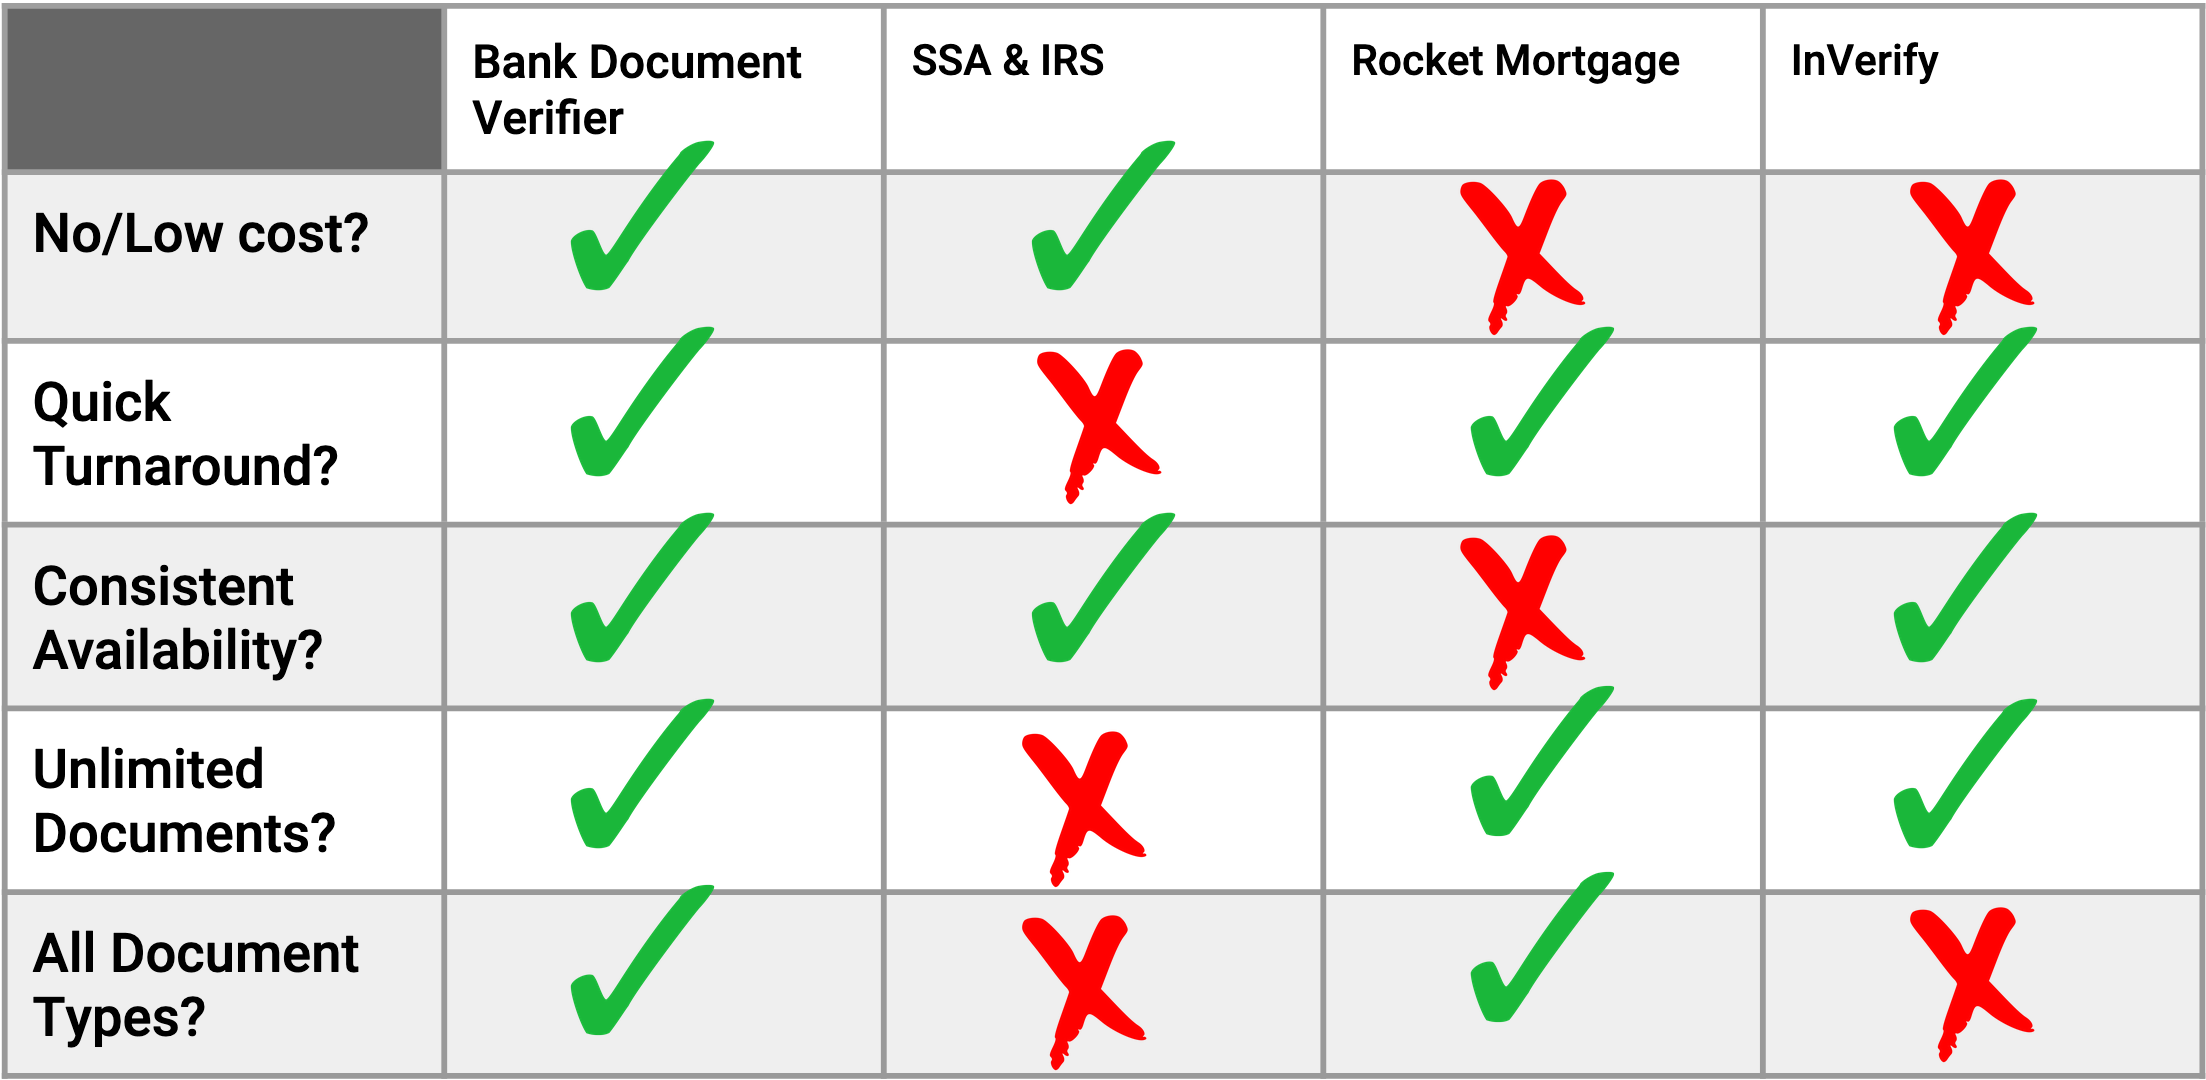
\includegraphics[width=0.48\textwidth]{assets/comparison-table.png}
    \caption{How our system compares with others}
\end{wrapfigure}

Humans are prone to inane mistakes and are thousands of times slower than a computer is. As such, there do exist verification systems out there. But most of them have issues with either speed, consistency, or generality. Our customer base is going to need a plethora of documents to be verified and, as such, we want to be able to scan all of them efficiently. Many of the current products will scan fast and accurately, but those tend to not scan all document types. The SSA and IRS also offer options, but they limit how many documents can be verified at once and are extremely slow. We believe the Bank Document Verifier will be able to cover what these other companies have lacked.

\subsection{Required Technology}

In order to create a modern, flexible, tried-and-tested, and secure Windows 10 desktop application, it is essential that we thoughtfully consider frameworks and platforms that fit this requirement. For this, we have been considering modern frameworks and platforms that support cross-platform development but could still be built specifically with Windows 10 in mind. After extensive research, we determined that React Native would be an excellent option as a development framework for our front-end. Some advantages of React Native include: 

\begin{itemize}
    \item Support for the Universal Windows Platform, allowing for better permissions management, easy installation/uninstallation, and adaptation to different device screen sizes, resolutions, and DPIs
    \item Optimal performance/stability
    \item A modular architecture, allowing for free and interchangeable functions which we can reuse across the code base.
    \item A large community of support, showing that the framework is clearly tried-and-tested
    \item The ability for cross-platform development, in case we want to develop for Linux or macOS.
\end{itemize}

The back-end will be written in both Node.js and Python, where we will be using Python to handle anything that might be and Node.js to handle strict I/O operations, as each platform suits its respective task well.

\subsection{Assets}

There is an API called Accurint that can be used to verify many forms of identification. Many of the projects we saw in our research used that to a high degree of success but stopped short of having all the features we’d like.

\subsection{Hardware/Software Requirements}

Due to our program’s ease of incorporation into current financial institutions, as well as its relative programmatic simplicity, we will not require any hardware or software beyond what the institution already has in each of its computers (Windows 10, a mid-range processor, and, comfortably, 4 GB+ of RAM as well as 5 GB+ of storage).   